%%%%%%%%%%%%%%%%%%%%%%%%%%%%%%%%%%%%%%%%%%%%%%%%%%%%%%%%%%%%%%%%%%%%%%%%%%%%%%%
\documentclass[hyperref={pdfpagelabels=false},compress,table]{beamer} % 在Mac下无法编译
% \documentclass[compress,table]{beamer} % 在Mac下使用
% package for font
\usepackage{fontspec}
\defaultfontfeatures{Mapping=tex-text}  %%如果没有它,会有一些 tex 特殊字符无法正常使用,比如连字符。
\usepackage{xunicode,xltxtra}
\usepackage[BoldFont,SlantFont,CJKnumber,CJKchecksingle]{xeCJK}  % \CJKnumber{12345}: 一万二千三百四十五
\usepackage{CJKfntef}  %%实现对汉字加点、下划线等。
\usepackage{pifont}  % \ding{}
% package for math
\usepackage{amsfonts}

% package for graphics
\usepackage[americaninductors,europeanresistors]{circuitikz}
\usepackage{tikz}
\usetikzlibrary{plotmarks}  % placements=positioning
\usepackage{graphicx}  % \includegraphics[]{}
\usepackage{subfigure}  %%图形或表格并排排列
% package for table
\usepackage{colortbl,dcolumn}  %% 彩色表格
\usepackage{multirow}
\usepackage{multicol}
\usepackage{booktabs}
% package for code
\usepackage{fancyvrb}
\usepackage{listings}

% \usepackage{animate}
% \usepackage{movie15}

%%%%%
% setting for beamer
\usetheme{default} % Madrid(常用), Copenhagen, AnnArbor, boxes(白色), Frankfurt,Berkeley
\useoutertheme[subsection=true]{miniframes} % 使用Berkeley时注释本行
\usecolortheme{sidebartab}
\usefonttheme{serif}  %%英文使用衬线字体
% \setbeamertemplate{background canvas}[vertical
% shading][bottom=white,top=structure.fg!7] %%背景色,上25%的蓝,过渡到下白。
\setbeamertemplate{theorems}[numbered]
\setbeamertemplate{navigation symbols}{}  %% 去掉页面下方默认的导航条
\setbeamercovered{transparent}  %设置 beamer 覆盖效果

% 设置标题title背景色
% \setbeamercolor{title}{fg=black, bg=lightgray!60!white}
\setbeamercolor{title}{fg=white, bg=black!70!white}

% 设置每页小LOGO
\pgfdeclareimage[width=1cm]{ouc}{figures/static/ouc.pdf}
\logo{\pgfuseimage{ouc}{\vspace{-20pt}}}

% setting for font
%%\setCJKmainfont{Adobe Kaiti Std}
\setCJKmainfont{SimSun} 
%% \setCJKmainfont{FangSong_GB2312} 
%% \setmainfont{Apple Garamond}  %%苹果字体没有SmallCaps
\setCJKmainfont{SimSun} 
%FUNNY%\setCJKmainfont{DFPShaoNvW5-GB}  %%华康少女文字W5(P)
%FUNNY%\setCJKmainfont{FZJingLeiS-R-GB}  %%方正静蕾体
%FUNNY%\setmainfont{Purisa}
%\setsansfont[Mapping=tex-text]{Adobe Song Std}
     %如果装了Adobe Acrobat,可在font.conf中配置Adobe字体的路径以使用其中文字体。
     %也可直接使用系统中的中文字体如SimSun、SimHei、微软雅黑等。
     %原来beamer用的字体是sans family;注意Mapping的大小写,不能写错。
     %设置字体时也可以直接用字体名,以下三种方式等同:
     %\setromanfont[BoldFont={黑体}]{宋体}
     %\setromanfont[BoldFont={SimHei}]{SimSun}
     %\setromanfont[BoldFont={"[simhei.ttf]"}]{"[simsun.ttc]"}
% setting for graphics
\graphicspath{{figures/}}  %%图片路径
\renewcommand\figurename{图}

% setting for pdf
\hypersetup{% pdfpagemode=FullScreen,%
            pdfauthor={Xiaodong Wang},%
            pdftitle={Title},%
            CJKbookmarks=true,%
            bookmarksnumbered=true,%
            bookmarksopen=false,%
            plainpages=false,%
            colorlinks=true,%
            citecolor=green,%
            filecolor=magenta,%
            linkcolor=blue,%red(default)
            urlcolor=cyan}

% setting for fontspec
\XeTeXlinebreaklocale "zh"  %%表示用中文的断行
\XeTeXlinebreakskip = 0pt plus 1pt minus 0.1pt  %%多一点调整的空间
%%%%%

% font setting by xeCJK
\setCJKfamilyfont{NSimSun}{NSimSun}
\newcommand{\song}{\CJKfamily{NSimSun}}
%%%\setCJKfamilyfont{AdobeSongStd}{Adobe Song Std}
%%%\newcommand{\AdobeSong}{\CJKfamily{AdobeSongStd}}
\setCJKfamilyfont{FangSong}{FangSong_GB2312}
\newcommand{\fang}{\CJKfamily{FangSong}}
%%%\setCJKfamilyfont{AdobeFangsongStd}{Adobe Fangsong Std}
%%%\newcommand{\AdobeFang}{\CJKfamily{AdobeFangsongStd}}
\setCJKfamilyfont{SimHei}{SimHei}
\newcommand{\hei}{\CJKfamily{SimHei}}
%%%\setCJKfamilyfont{AdobeHeitiStd}{Adobe Heiti Std}
%%%\newcommand{\AdobeHei}{\CJKfamily{AdobeHeitiStd}}
\setCJKfamilyfont{KaiTi}{KaiTi}
\newcommand{\kai}{\CJKfamily{KaiTi}}
%%%\setCJKfamilyfont{AdobeKaitiStd}{Adobe Kaiti Std}
\newcommand{\AdobeKai}{\CJKfamily{AdobeKaitiStd}}
\setCJKfamilyfont{LiSu}{LiSu}
\newcommand{\li}{\CJKfamily{LiSu}}
\setCJKfamilyfont{YouYuan}{YouYuan}
\newcommand{\you}{\CJKfamily{YouYuan}}
\setCJKfamilyfont{FZJingLei}{FZJingLeiS-R-GB}
\newcommand{\jinglei}{\CJKfamily{FZJingLei}}
\setCJKfamilyfont{MSYH}{Microsoft YaHei}
\newcommand{\msyh}{\CJKfamily{MSYH}}

% 自定义颜色
\def\Red{\color{red}}
\def\Green{\color{green}}
\def\Blue{\color{blue}}
\def\Mage{\color{magenta}}
\def\Cyan{\color{cyan}}
\def\Brown{\color{brown}}
\def\White{\color{white}}
\def\Black{\color{black}}

\lstnewenvironment{xmlCode}[1][]{% for Java
  \lstset{
    basicstyle=\tiny\ttfamily,%
    columns=flexible,%
    framexleftmargin=.7mm, %
    % frame=shadowbox,%
    % rulesepcolor=\color{cyan},%
     frame=single,%
    backgroundcolor=\color{white},%
    xleftmargin=4\fboxsep,%
    xrightmargin=4\fboxsep,%
    numbers=left,numberstyle=\tiny,%
    numberblanklines=false,numbersep=7pt,%
    language=xml, %
    }\lstset{#1}}{}

\lstnewenvironment{javaCode}[1][]{% for Java
  \lstset{
    basicstyle=\tiny\ttfamily,%
    columns=flexible,%
    framexleftmargin=.7mm, %
    frame=shadowbox,%
    rulesepcolor=\color{cyan},%
    % frame=single,%
    backgroundcolor=\color{white},%
    xleftmargin=4\fboxsep,%
    xrightmargin=4\fboxsep,%
    numbers=left,numberstyle=\tiny,%
    numberblanklines=false,numbersep=7pt,%
    language=Java, %
    }\lstset{#1}}{}

\lstnewenvironment{shCode}[1][]{% for Java
  \lstset{
    basicstyle=\scriptsize\ttfamily,%
    columns=flexible,%
    framexleftmargin=.7mm, %
    frame=shadowbox,%
    rulesepcolor=\color{brown},%
    % frame=single,%
    backgroundcolor=\color{white},%
    xleftmargin=4\fboxsep,%
    xrightmargin=4\fboxsep,%
    numbers=left,numberstyle=\tiny,%
    numberblanklines=false,numbersep=7pt,%
    language=sh, %
    }\lstset{#1}}{}

\newcommand\ask[1]{\vskip 4bp \tikz \node[rectangle,rounded corners,minimum size=6mm,
  fill=white,]{\Cyan \includegraphics[height=1.5cm]{question} \Large \msyh #1};}

\newcommand\wxd[1]{\vskip 4bp \tikz \node[rectangle,minimum size=6mm,
  fill=blue!60!white,]{\White \ding{118} \msyh #1};}

\newcommand\xyy[1]{\vskip 2bp \tikz \node[rectangle,minimum size=3mm,
  fill=black!80!white,]{\White \msyh\scriptsize #1};}

\newcommand\cxf[1]{\vskip 4bp \tikz \node[rectangle,rounded corners,minimum size=6mm,
  fill=orange!60!white,]{\White \ding{42} \msyh #1};}

\newcommand\samp[1]{\vskip 2bp \tikz \node[rectangle,minimum size=3mm,
  fill=white!100!white,]{\Mage\msyh \small CODE \ding{231} \Black #1};\vskip -8bp}

\newcommand\zhyfly[1]{\tikz \node[rectangle,rounded corners,minimum size=6mm,ball color=red!25!blue,text=white,]{#1};}

\setbeamerfont{frametitle}{series=\msyh} % 修改Beamer标题字体

\makeatletter
\newcommand{\Extend}[5]{\ext@arrow 0099{\arrowfill@#1#2#3}{#4}{#5}}
\makeatother


%%%%%%%%%%%%%%%%%%%%%%%%%%%%%%%%%%%%%%%%%%%%%%%%%%%%%%%%%%%%%%%%%%%%%%%%%%%%%%%
% \titlepage
\title[KevinW@OUC]{\hei {\huge Java应用与开发}\\  
  MVC和框架初步}
\author[王晓东]{王晓东\\
  \href{mailto:wangxiaodong@ouc.edu.cn}{\footnotesize wangxiaodong@ouc.edu.cn}}
\institute[中国海洋大学]{\small 中国海洋大学}
\date{\today}
\titlegraphic{\vspace{-6em}
\includegraphics[height=6cm]{static/ouc.pdf}\vspace{-6em}}
%%%%%
\begin{document}
%% Delete this, if you do not want the table of contents to pop up at
%% the beginning of each subsection:
\AtBeginSection[]{                              % 在每个Section前都会加入的Frame
  \frame<handout:0>{
    \frametitle{\textbf{\hei 接下来…}}
    \tableofcontents[currentsection]
  }
}  %

\AtBeginSubsection[]                            % 在每个子段落之前
{
  \frame<handout:0>                             % handout:0 表示只在手稿中出现
  {
    \frametitle{\textit{\hei 接下来…}}\small
    \tableofcontents[current,currentsubsection] % 显示在目录中加亮的当前章节
  }
}
 \frame{\titlepage}


%%%%%%%%%%%%%%%%%%%%%%%%%%%%%%%%%%%%%%%%%%%%%%%%
\begin{frame}
\frametitle{学习目标}
\begin{enumerate}
\item 理解MVC设计模式的概念与特点,初步认识框架产生的基础。
\item 了解经典的MVC框架——Struts 2,学会使用Eclipse入手编写一个Struts 2
  Web应用。
\item 通过Struts 2的经典MVC框架设计和业务代码开发过程,进一步思考、理解
  框架。
\end{enumerate}  
\end{frame}
 
%%%%%%%%%%%%%%%%%%%%%%%%%%%%%%%%%%%%%%%%%%%%%%%%
\section*{大纲}
\frame{\frametitle{大纲} \tableofcontents }

\section{Java Web应用的开发演化}

\begin{frame}[fragile] % [fragile]参数使得能够插入代码
\frametitle{JSP方式}

JSP在HTML代码里写Java代码完成业务逻辑。

\begin{xmlCode}
<%
     String name = request.getParameter("name");
     String password = request.getParameter("password");

     UserHandler userHandler = new UserHandler();
     if(userHandler.authenticate(name, password)) {
%>
<p>Congratulations, login successfully. </p>
<%
      } else {
%>
<p>Sorry, login failed.</p>
<%
      }
%>
\end{xmlCode}
\end{frame}

\begin{frame}[fragile] % [fragile]参数使得能够插入代码
\frametitle{JSP方式}

\wxd{仅有的一点优势}\kai
\begin{enumerate}
\item 无需额外的配置文件,无需框架的帮助,即可完成逻辑。
\item 简单易上手。
\end{enumerate}

\wxd{劣势}
\begin{enumerate}[<+-| alert@+>]\kai
\item Java代码由于混杂在一个HTML环境中而显得混乱不堪,可读性非常差。一个JSP文件有时候会变
  成几十K,甚至上百K,经常难以定位逻辑代码的所在。
\item 编写代码时非常困惑,不知道代码到底应该写在哪里,也不知道别人是不是已经曾经实现过类
  似的功能,到哪里去引用。
\item 突然之间,某个需求发生了变化。于是,每个人蒙头开始全程替换,还要小心翼翼的,生怕把
  别人的逻辑改了。
\item 逻辑处理程序需要自己来维护生命周期,对于类似数据库事务、日志等众多模块无法统一支
  持。
\end{enumerate}
\end{frame}

\begin{frame}[fragile] % [fragile]参数使得能够插入代码
\frametitle{需求的变化}

\begin{itemize}
\item 在这个时候,如果有一种方式,它能够将页面上的那些Java代码抽取出来,
  让页面上尽量少出现Java代码,该有多好。
\item {\Blue\hei 于是许多人开始使用servlet来处理那些业务逻辑。 }
\end{itemize}


\end{frame}

\begin{frame}[fragile] % [fragile]参数使得能够插入代码
\frametitle{Servlet方式}

\begin{javaCode}
public class LoginServlet extends HttpServlet {
  
  @Override
  protected void doPost(HttpServletRequest req, HttpServletResponse resp) 
  throws ServletException, IOException {
    String message = null;
    RequestDispatcher dispatcher = req.getRequestDispatcher("/result.jsp");
    String name = req.getParameter("name");
    String password = req.getParameter("password");
    
    UserHandler userHandler = new UserHandler();
    if(userHandler.authenticate(name, password)) {
      message = "恭喜你,登录成功";
    } else {
      message = "对不起,登录失败";
    }
    
    req.setAttribute("message", message);
    dispatcher.forward(req, resp);
  }
}
\end{javaCode}
\end{frame}

\begin{frame}[fragile] % [fragile]参数使得能够插入代码
  \frametitle{框架方式}

  \begin{itemize}
  \item 时代进一步发展,人们发现简单的JSP和Servlet已经很难满足人们懒惰的
    要求。于是,人们开始试图总结一些公用的Java类,来解决Web开发过程中碰到
    的问题。这时,横空出世了一个框架,叫做{\bf\Red Struts}。它非常先进地实现
    了{\hei\Red MVC模式},成为了广大程序员的福音。
  \item 在一定程度上,Struts能够解决Web开发中的职责分配问题,使得显示与逻
    辑分开。
  \item {\Blue\kai 不过开始的在很长一段时间里,学习使用Struts的程序员往
      往无法清晰的明白我们到底需要Web框架帮我们做什么,我们到底需要它完
      成点什么功能。}
  \end{itemize}
\end{frame}

\begin{frame}[fragile] % [fragile]参数使得能够插入代码
\frametitle{那么我们需要什么?}

在回顾写代码的历史之后,回头来看看,我们到底需要什么? 

无论是使用JSP,还是使用Struts1,或是Struts2,我们至少都需要一些必须的元素(如果没有这些元
素,或许我还真不知道这个程序会写成什么样子):

\begin{enumerate}[<+-| alert@+>]
\item {\hei 数据} \only<1>{在用户登录实例中就是name和password。他们共同
    构成了程序数据的核心载体。事实上,我们往往会有一个User类来封
    装name和password,这样会使得我们的程序更加OO。无论怎么说,数据会穿
    插在这个程序的各处,成为程序运行的核心。 }
\item {\hei 页面展示} \only<2>{例如用户登录页面login.jsp。没有这个页面,
    一切的请求、验证和错误展示也无从谈起。在页面上,我们需要利用HTML,
    把我们需要展现的数据都呈现出来。同时我们也需要完成一定的页面逻辑,
    例如,错误展示,分支判断等。 }
\item {\hei 处理具体业务的场所} \only<3>{不同阶段,处理具体业务的场所就
    不太一样。原来用JSP和Servlet,后来用Struts1或者Struts2的Action。}
\end{enumerate}
\end{frame}

\begin{frame}[fragile] % [fragile]参数使得能够插入代码
  \frametitle{MVC}

  以上这些必须出现的元素,在不同的时代被赋予了不同的表现形式,有的受到
  时代的束缚,其表现形式非常落后,有的已经不再使用。但是拨开这些外在的
  表现形式,我们就可以发现,这就是我们已经熟悉的MVC。

  \begin{itemize}
  \item 数据 \ding{235} Model 
  \item 页面展示 \ding{235} View 
  \item 处理具体业务的场所 \ding{235} Control 
  \end{itemize}

  {\hei\Red 框架不重要。只要能够深刻理解MVC的概念,框架只是几个jar包而已。}
\end{frame}

\begin{frame}[fragile] % [fragile]参数使得能够插入代码
\frametitle{MVC}

\begin{figure}
\centering
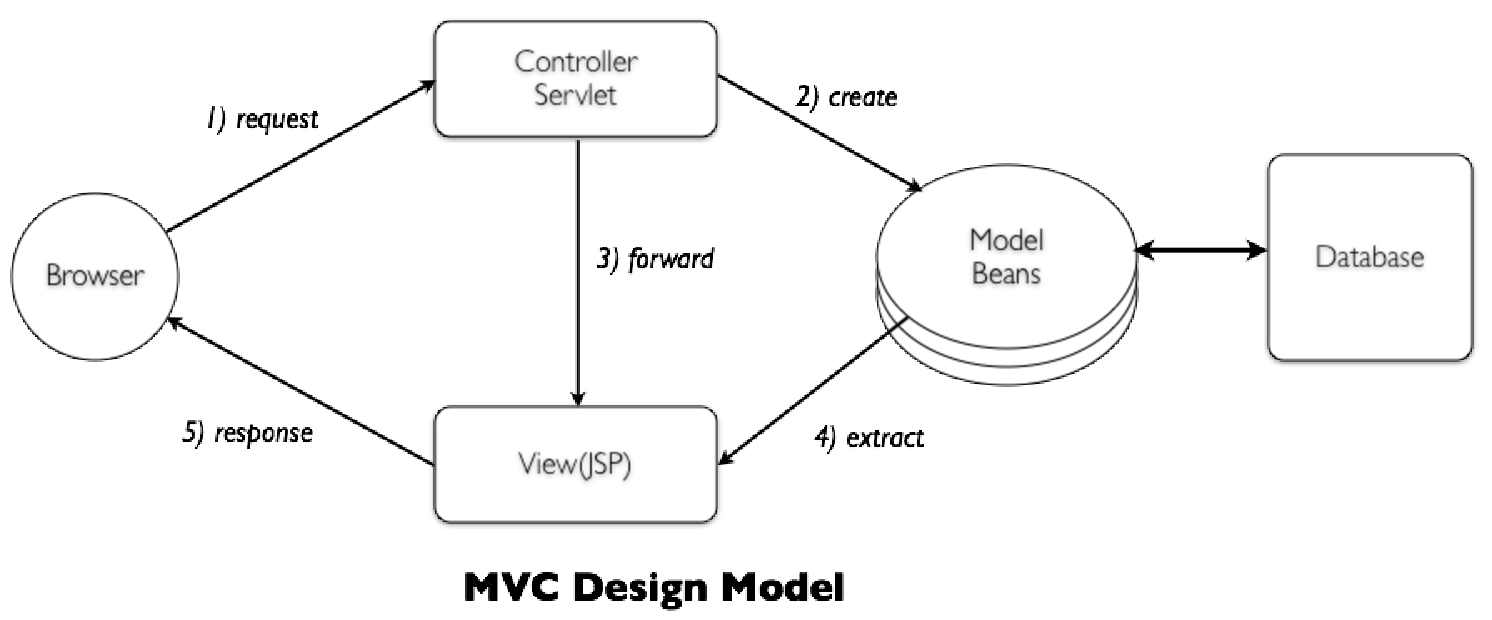
\includegraphics[width=0.9\textwidth]{fig02.pdf}
\end{figure}
\end{frame}

\begin{frame}[fragile] % [fragile]参数使得能够插入代码
  \frametitle{MVC的特点}\kai
  \begin{enumerate}
  \item 多个视图可以对应一个模型,可以减少代码的复制,在模型发生改变时,易于维护。
  \item 模型返回的数据与显示逻辑分离。模型数据可以应用任何显示技术,例如,使用JSP、Velocity模板或者直接产生Excel。
  \item 应用被分为三层,降低各层耦合,提高了可扩展性。
  \item 控制层把不同模型和视图组合在一起,完成不同的请求,控制层包含了用户请求权限的概念。
  \item MVC符合软件工程化管理的思想,不同层各司其职,有利于通过工程化和工具化产生管理程序代码。
  \end{enumerate}
\end{frame}

\begin{frame}[fragile] % [fragile]参数使得能够插入代码
  \frametitle{MVC}

  数据是动的,数据在View和Control层一旦运动起来,就会产生许多的问题:
  \begin{itemize}[<+-| alert@+>]\kai\small
  \item 数据从View层传递到Control层,如何使得一个个扁平的字符串,转化成一个个生龙活虎的Java对象。
  \item 数据从View层传递到Control层,如何方便的进行数据格式和内容的校验? 
  \item 数据从Control层传递到View层,一个个生龙活虎的Java对象,又如何在页面上以各种各样的形式展现出来 。
  \item 如果你试图将数据请求从View层发送到Control层,你如何才能知道你要调用的究竟是哪个类,
    哪个方法?一个HTTP的请求,又如何与Control层的Java代码建立起关系来?
  \end{itemize}
\end{frame}

\begin{frame}[fragile] % [fragile]参数使得能够插入代码
\frametitle{框架}

框架是为了解决一个又一个在Web开发中所遇到的问题而诞生的。不同的框架,都
是为了解决不同的问题,但是对于程序员而言,他们仅仅是jar包而已。框架的优
缺点的评论,也完全取决于其对问题解决程度和解决方式的优雅性的评论。

所以,{\hei\Blue 千万不要为了学习框架而学习框架,而是要为了解决问题而学
  习框架,这才是一个程序员的正确学习之道 。}
\end{frame}

\section{经典MVC框架 - Struts 2}

\subsection{为Web应用增加Struts 2支持}

\begin{frame}[fragile] % [fragile]参数使得能够插入代码
  \frametitle{为Web应用增加Struts 2支持}
  
  \begin{enumerate}%\setcounter{enumi}{1-1} % n-1,从n开始
  \item 下载安装Struts 2,登录http://struts.apache.org/download.cgi,下
    载Struts 2的完整版(Full Distribution)。此处版本
    为:struts-2.3.15.1-all.zip。
  \end{enumerate}

  \begin{shCode}
    [18:10]xiaodong@Wang:~/Installed/struts-2.3.15.1[0]
    > ls
    ANTLR-LICENSE.txt       OGNL-LICENSE.txt        apps
    CLASSWORLDS-LICENSE.txt OVAL-LICENSE.txt        docs
    FREEMARKER-LICENSE.txt  SITEMESH-LICENSE.txt    lib
    LICENSE.txt             XPP3-LICENSE.txt        src
    NOTICE.txt              XSTREAM-LICENSE.txt
  \end{shCode}
\end{frame}

\begin{frame}[fragile] % [fragile]参数使得能够插入代码
\frametitle{为Web应用增加Struts 2支持}
\begin{enumerate}\setcounter{enumi}{1} % n-1,从n开始
\item 将Struts 2的lib目录下的{\Red\bf
    commons-fileupload-*.jar、commons-io-*.jar、freemarker-*.jar、
    javassist-*.jar、ognl-*.jar、struts2-core-*.jar、xwork-core-*.jar}
  必备类库复制到{\bf\Red Web应用的WEB-INF/lib路径下}。

  如果需要在DOS或Shell窗口下手动编译Strut 2相关程序,还需要
  将struts2-core-*.jar和xwork-core-*.jar添加到系统的CLASSPATH环境变量。
\end{enumerate}
\end{frame}

\begin{frame}[fragile] % [fragile]参数使得能够插入代码
  \frametitle{为Web应用增加Struts 2支持}
  
  \begin{enumerate}\setcounter{enumi}{2} % n-1,从n开始
  \item 编辑Web应用的web.xml配置文件,配置Strut 2的核心过滤器(Filter)。

    \begin{xmlCode}\footnotesize
      <?xml version="1.0" encoding="GBK"?>
      <web-app xmlns:xsi="http://www.w3.org/2001/XMLSchema-instance" 
      xmlns="http://java.sun.com/xml/ns/javaee" 
      xmlns:web="http://java.sun.com/xml/ns/javaee/web-app_2_5.xsd" 
      xsi:schemaLocation="http://java.sun.com/xml/ns/javaee 
      http://java.sun.com/xml/ns/javaee/web-app_3_0.xsd" 
      id="WebApp_ID" version="3.0">

        <!-- 定义 Struts2 的核心 Filter -->
        <filter>
          <filter-name>struts2</filter-name>
          <filter-class>org.apache.struts2.dispatcher.ng.filter.
            StrutsPrepareAndExecuteFilter</filter-class>
        </filter>
        
        <!-- 让Struts2 的核心 Filter 拦截所有请求 -->
        <filter-mapping>
          <filter-name>struts2</filter-name>
          <url-pattern>/*</url-pattern>
        </filter-mapping>
      </web-app>   
    \end{xmlCode}
\end{enumerate}
\end{frame}

\begin{frame}[fragile] % [fragile]参数使得能够插入代码
  \frametitle{为Web应用增加Struts 2支持}

  \begin{enumerate}\setcounter{enumi}{3} % n-1,从n开始
  \item 使用Struts 2的功能需要一个struts.xml配置文件,默认放在Web应用的类加载路径下(通常是WEB-INF/classes)。
  \end{enumerate}

  经过上述步骤,我们可以在一个Web应用中使用Struts 2的基本功能。
\end{frame}

\subsection{在Eclipse中使用Struts 2}

\begin{frame}[fragile] % [fragile]参数使得能够插入代码
  \frametitle{创建并配置项目}

  在Eclipse中创建动态Web项目:sample.struts2,按照上述步骤配置该项目。主要包括:

  \begin{itemize}
  \item 添加依赖的Struts 2类库;
  \item 在web.xml中加入并配置核心过滤器。
  \end{itemize}

\end{frame}

\begin{frame}[fragile] % [fragile]参数使得能够插入代码
\frametitle{增加登录处理}

以下示例为sample.struts2应用增加一个简单的登录处理流程,以简要介绍Struts 2的开发步骤。

\wxd{编写JSP页面}

File: sample.struts2/WebContent/login.jsp

\begin{xmlCode}
  <%@ page language="java" contentType="text/html; charset=UTF-8"
    pageEncoding="UTF-8"%>
  <%@taglib prefix="s" uri="/struts-tags"%>
  <!DOCTYPE html>
  <html>
  <head>
    <meta charset="UTF-8">
    <title><s:text name="loginPage" /></title>
  </head>
  <body>
    <h2>用户登录</h2>
    <s:form action="login">
      <s:textfield name="username" key="user"/>
      <s:password name="password" key="pass"/>
      <s:submit key="login"/>
    </s:form>
  </body>
  </html>  
\end{xmlCode}
\end{frame}

\begin{frame}[fragile] % [fragile]参数使得能够插入代码
\frametitle{增加登录处理}

上述login.jsp页面使用Struts 2标签库定义了一个表单和三个简单表单域。

\notice{注意}

几乎所有的MVC框架都会使用标签库,用以帮助开发者更加简单、更加规范的编写
视图组件(例如JSP页面)。


\end{frame}

\begin{frame}[fragile] % [fragile]参数使得能够插入代码
\frametitle{增加登录处理}

提供welcome.jsp页面和error.jsp页面,作为登录成功、登录失败后的提示页
面。

\ttc{sample.struts2/WebContent/welcome.jsp}

{\footnotesize\Blue
\begin{verbatim}
<body>
  <s:text name="succTip">
    <s:param>${sessionScope.user}</s:param>
  /s:text><br/>
</body>
\end{verbatim}}

\ttc{sample.struts2/WebContent/error.jsp}

{\footnotesize\Blue
\begin{verbatim}
<body>
  <s:text name="failTip"/>
</body>
\end{verbatim}}
\end{frame}

\begin{frame}[fragile] % [fragile]参数使得能够插入代码
  \frametitle{增加登录处理}

  为了让Struts 2运行起来,还必须为Struts 2框架提供一个配置文件:{\bf\Red struts.xml}。

  \ttc{sample.struts2/{\Red src}/struts.xml}

  \begin{xmlCode}
    <?xml version="1.0" encoding="UTF-8"?>
    <!DOCTYPE struts PUBLIC
    "-//Apache Software Foundation//DTD Struts Configuration 2.1.7//EN"
    "http://struts.apache.org/dtds/struts-2.1.7.dtd">
    <!-- 指定 Struts 2 配置文件的根元素 -->
    <struts>
      <!-- 指定全局国际化资源文件 -->
      <constant name="struts.custom.i18n.resources" value="mess"/>
      <!-- 指定国际化编码所使用的字符集 -->	
      <constant name="struts.i18n.encoding" value="UTF-8"/>
      ...
    </struts>  
  \end{xmlCode}

  {\kai\Blue 注意:在Eclipse的管理下,当Eclipse生成、部署Web项目时,会
    自动将src路径下除了*.java外所有的文件都复制到Web应用
    的WEB-INF/classes路径下,所以struts.xml文件可以放在src目录。}

\end{frame}
\begin{frame}[fragile] % [fragile]参数使得能够插入代码
\frametitle{增加登录处理}

上述struts.xml文件中制定了国际化资源文件的base名为mess,所以需要为该应
用提供一个mess\_zh\_CN.properties文件。

\ttc{sample.struts2/src/mess\_XXX\_XXX.properties}

\begin{xmlCode}
loginPage = 登录页面
errorPage = 错误页面
succPage = 成功页面
failTip = 对不起,您不能登录!
succTip = 欢迎, {0} ,您已经登录!
user = 用户名
pass = 密码
login = 登录
\end{xmlCode}

必须用native2ascii命令处理该国际化资源文件(Eclipse中自动完成)

\end{frame}

\begin{frame}[fragile] % [fragile]参数使得能够插入代码
\frametitle{增加登录处理}

login.jsp页面中登录表单时指定改表单的action为login,所以必须定义一个Struts
2的Action,通常该继承ActionSupport基类。
\end{frame}

\begin{frame}[fragile] % [fragile]参数使得能够插入代码
\frametitle{增加登录处理}

\ttc{sample.struts2/src/ouc/java/app/action/LoginAction.java}

\begin{javaCode}
  public class LoginAction extends ActionSupport {
    // 定义封装请求参数的 username 和 password 属性
    private String username;
    private String password;
    public String getUsername() {
      return username;
    }
    public void setUsername(String username) {
      this.username = username;
    }
    public String getPassword() {
      return password;
    }
    public void setPassword(String password) {
      this.password = password;
    }
    // 定义处理用户请求的 execute 方法
    public String execute() throws Exception {
      if (getUsername().equals("admin") && getPassword().equals("admin")) {
        ActionContext.getContext().getSession().put("user", getUsername());
        return SUCCESS;
      } else {
        return ERROR;
      }
    }
  }
\end{javaCode}
\end{frame}

\begin{frame}[fragile] % [fragile]参数使得能够插入代码
\frametitle{增加登录处理}

\ttc{在struts.xml中配置action}

\begin{xmlCode}
... ...
<struts>
  <!-- 指定全局国际化资源文件 -->
  <constant name="struts.custom.i18n.resources" value="mess"/>
  <!-- 指定国际化编码所使用的字符集 -->	
  <constant name="struts.i18n.encoding" value="GBK"/>
  <!-- 所有的 Action 定义都应该放在 package 下 -->
  <package name="oucj2ee" extends="struts-default">
    <action name="login" class="ouc.java.app.action.LoginAction">
    <!-- 定义三个逻辑视图和物理资源之间的映射 -->		
      <result name="input">/login.jsp</result>
      <result name="error">/error.jsp</result>
      <result name="success">/welcome.jsp</result>
    </action>
  </package>
</struts>
\end{xmlCode}

{\Blue\kai 配置一个名称为login的Action,该Action配置三个result元素,用
  于指定逻辑视图与物理资源之间的映射。例如,当返回input逻辑视图名称时,
  系统跳转到/login.jsp页面。}
\end{frame}

\subsection{Struts 2的开发步骤小结}

\begin{frame}[fragile] % [fragile]参数使得能够插入代码
\frametitle{\ding{182} 在web.xml中配置核心过滤器}

在web.xml文件中增加如下配置片段:

\begin{xmlCode}
<!-- 定义 Struts 2 的核心过滤器 -->
<filter>
  <filter-name>struts2</filter-name>
  <filter-class>
    org.apache.struts2.dispatcher.ng.filter.StrutsPrepareAndExecuteFilter
  </filter-class>
</filter>
<!-- 让 Struts 2 的核心过滤器拦截所有请求 -->
<filter-mapping>
  <filter-name>struts2</filter-name>
  <url-pattern>/*</url-pattern>
</filter-mapping>  
\end{xmlCode}

\end{frame}

\begin{frame}[fragile] % [fragile]参数使得能够插入代码
\frametitle{\ding{183} 定义包含表单数据的JSP页面}

\begin{itemize}
\item 如果以{\bf\Red POST}方式提交表单数据,则定义包含表单数据的JSP页
  面。
\item 如果仅仅以{\bf\Blue GET}方式发送请求,则无需经过这一步。
\end{itemize}
\end{frame}

\begin{frame}[fragile] % [fragile]参数使得能够插入代码
\frametitle{\ding{184} 定义处理用户请求的Action类}

\begin{itemize}
\item Action是MVC中的C,即控制器。
\item 控制器Action负责调用Model里的方法来处理请求。
\item 在Struts 2中,MVC框架控制器实际上由两个部分组成:
  \begin{enumerate}\kai
  \item 拦截所有用户请求,处理请求的通用代码由核心控制器完成;
\item 实际业务控制则有Action处理。
\end{enumerate}

\end{itemize}

{\Blue\kai\scriptsize 注意:核心过滤器接收到用户请求后,通常会对用户请
  求进行简单预处理(例如解析、封装参数),然后通过反射来创建Action实例,
  并调用Action的指定方法(Struts 1通常是execute,Struts 2可以是任意方法)
  来处理用户请求。}
\end{frame}

\begin{frame}[fragile] % [fragile]参数使得能够插入代码
\frametitle{\ding{185} 在struts.xml中配置Action}

通常采用如下XML片段配置Action:

\begin{xmlCode}
<action name="login" class="ouc.java.app.action.LoginAction">
  ... ...
</action>
\end{xmlCode}

上述配置指定:

用户请求的URL为login则使用ouc.java.app.action.LoginAction来处理。

{\Blue\kai\scriptsize 注意:现在Struts 2的Convension插件借鉴Rails框架的
  优点,开始支持“约定优于配置”的思想,即采用约定的方式来规定用户请求地
  址和Action之间的对应关系。}
\end{frame}

\begin{frame}[fragile] % [fragile]参数使得能够插入代码
\frametitle{\ding{186} 配置处理结果和物理视图资源之间的对应关系}
\begin{itemize}
\item 当Action处理用户请求结束后,通常会返回一个处理结果(通常使用简单
  的字符串),我们可以认为该名称是{\hei\Red 逻辑视图名}。
\item 逻辑视图名需要和指定的物理视图资源关联才有价值,所以我们需要配置
  处理结果之间的对应关系。

\begin{xmlCode}
<action name="login" class="ouc.java.app.action.LoginAction">
  <!-- 定义3个逻辑视图和物理视图资源之间的映射 -->
  <result name="input">/login.jsp</result>
  <result name="error">/error.jsp</result>
  <result name="success">/success.jsp</result>
</action>  
\end{xmlCode}
\end{itemize}
\end{frame}

\begin{frame}[fragile] % [fragile]参数使得能够插入代码
  \frametitle{\ding{187} 编写视图资源}

  如果一个Action需要把一些数据传给视图资源,则可以借助{\Red\hei OGNL表达式}。

  经过上述步骤后,我们基本完成了一个Struts 2处理流程的开发,即可以完整的执行一次HTTP请求/响
  应过程。
\end{frame}

\begin{frame}[fragile] % [fragile]参数使得能够插入代码
  \frametitle{Struts 2流程}
  \begin{figure}
    \centering
    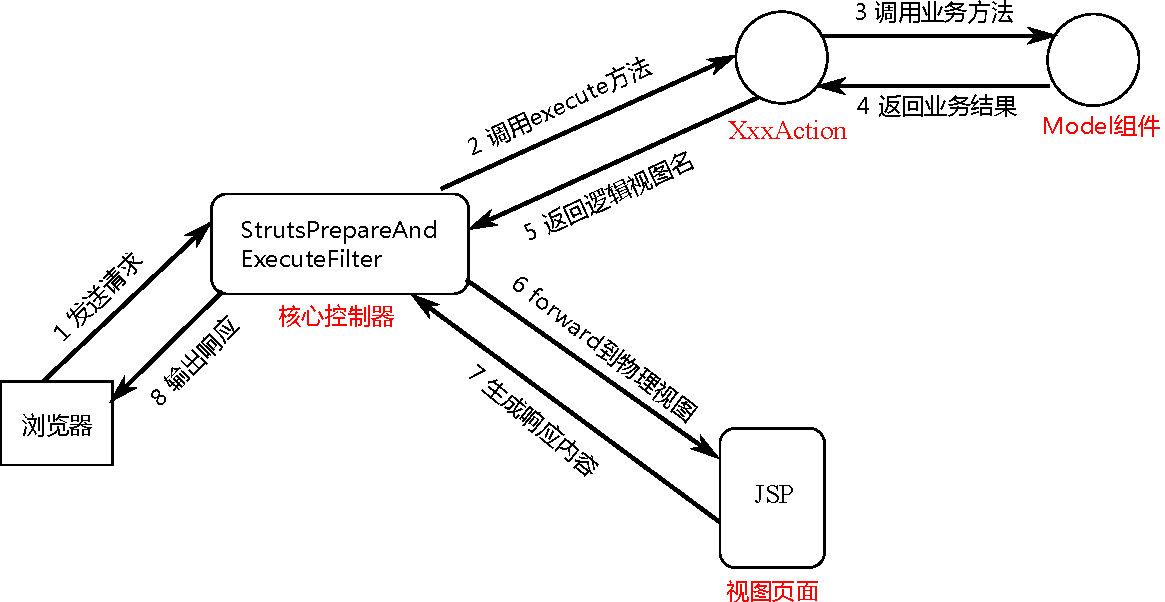
\includegraphics[width=0.8\textwidth]{fig01.pdf}
  \end{figure}
  \begin{itemize}\small\kai
  \item StrutsPrepareAndExecuteFilter和XxxAction共同构成Strut 2的控制器,其中前者称为核心控
    制器,后者称为业务控制器。
  \item 业务控制器并不与物理视图关联,这种做法提供了很好的解耦。
  \item 在Struts 2的控制下,用户请求不再向JSP页面发送,而是由核心控制器来“调用”JSP页面来生
    成响应,此处调用不是直接调用,而是将请求forward到指定的JSP页面。
  \end{itemize}
\end{frame}

\section{本节习题}

\begin{frame}
  \frametitle{本节习题}

  \tta{简答题}
  
  \begin{enumerate}
  \item 什么是MVC设计模式?
  \item MVC有哪些特点?
  \item 总结Struts 2 Web应用开发的主要步骤。
  \end{enumerate}
\end{frame}
  
\begin{frame}
  \frametitle{本节习题}
  
  \tta{小编程}

  \begin{enumerate}
  \item 参考幻灯片步骤实践Struts 2 Web应用开发实例,初步了解Struts 2和基本的MVC框架开发模式。
  \end{enumerate}
\end{frame}
% TKS %%%%%%%%%%%%%%%%%%%%%%%%%%%%%%%%%%%%%%%%%%%%%%
\begin{frame}
\centering
{\Huge \textcolor{blue}{THE END}} \\
\vspace{5mm}
{\Large wangxiaodong@ouc.edu.cn} \\
\end{frame}
%%%%%%%%%%%%%%%%%%%%%%%%%%%%%%%%%%%%%%%%%%%%%%%%%%
\end{document}
